%\documentclass[10pt,handout]{beamer}
\documentclass[10pt]{beamer}\usepackage[]{graphicx}\usepackage[]{color}
%% maxwidth is the original width if it is less than linewidth
%% otherwise use linewidth (to make sure the graphics do not exceed the margin)
\makeatletter
\def\maxwidth{ %
  \ifdim\Gin@nat@width>\linewidth
    \linewidth
  \else
    \Gin@nat@width
  \fi
}
\makeatother

\definecolor{fgcolor}{rgb}{0.345, 0.345, 0.345}
\newcommand{\hlnum}[1]{\textcolor[rgb]{0.686,0.059,0.569}{#1}}%
\newcommand{\hlstr}[1]{\textcolor[rgb]{0.192,0.494,0.8}{#1}}%
\newcommand{\hlcom}[1]{\textcolor[rgb]{0.678,0.584,0.686}{\textit{#1}}}%
\newcommand{\hlopt}[1]{\textcolor[rgb]{0,0,0}{#1}}%
\newcommand{\hlstd}[1]{\textcolor[rgb]{0.345,0.345,0.345}{#1}}%
\newcommand{\hlkwa}[1]{\textcolor[rgb]{0.161,0.373,0.58}{\textbf{#1}}}%
\newcommand{\hlkwb}[1]{\textcolor[rgb]{0.69,0.353,0.396}{#1}}%
\newcommand{\hlkwc}[1]{\textcolor[rgb]{0.333,0.667,0.333}{#1}}%
\newcommand{\hlkwd}[1]{\textcolor[rgb]{0.737,0.353,0.396}{\textbf{#1}}}%

\usepackage{framed}
\makeatletter
\newenvironment{kframe}{%
 \def\at@end@of@kframe{}%
 \ifinner\ifhmode%
  \def\at@end@of@kframe{\end{minipage}}%
  \begin{minipage}{\columnwidth}%
 \fi\fi%
 \def\FrameCommand##1{\hskip\@totalleftmargin \hskip-\fboxsep
 \colorbox{shadecolor}{##1}\hskip-\fboxsep
     % There is no \\@totalrightmargin, so:
     \hskip-\linewidth \hskip-\@totalleftmargin \hskip\columnwidth}%
 \MakeFramed {\advance\hsize-\width
   \@totalleftmargin\z@ \linewidth\hsize
   \@setminipage}}%
 {\par\unskip\endMakeFramed%
 \at@end@of@kframe}
\makeatother

\definecolor{shadecolor}{rgb}{.97, .97, .97}
\definecolor{messagecolor}{rgb}{0, 0, 0}
\definecolor{warningcolor}{rgb}{1, 0, 1}
\definecolor{errorcolor}{rgb}{1, 0, 0}
\newenvironment{knitrout}{}{} % an empty environment to be redefined in TeX

\usepackage{alltt}
\usepackage{etex} % helps fix \newdimen error which is cause when ctable is loaded with other packages
\usepackage{comment}
\usepackage{ctable}
\usepackage{amsmath,amsthm,amssymb}
\usepackage{url}
\usepackage{color, colortbl}
\usepackage{tikz}
\usetikzlibrary{shapes.geometric, arrows,shapes.symbols,decorations.pathreplacing}
\tikzstyle{startstop} = [rectangle, rounded corners, minimum width=3cm, minimum height=1cm,text centered, draw=black, fill=red!30,text width=2.0cm]
\tikzstyle{io} = [trapezium, trapezium left angle=70, trapezium right angle=110, minimum width=2cm, minimum height=1cm, text centered, draw=black, fill=blue!30,text width=1.5cm]
\tikzstyle{process} = [rectangle, minimum width=1cm, minimum height=1cm, text centered, draw=black, fill=orange!30,text width=2cm]
\tikzstyle{decision} = [diamond, minimum width=2cm, minimum height=1cm, text centered, draw=black, fill=green!30]
\tikzstyle{arrow} = [thick,->,>=stealth]
\tikzstyle{both} = [thick,<->,>=stealth, red]

\tikzset{myshade/.style={minimum size=.4cm,shading=radial,inner color=white,outer color={#1!90!gray}}}
\newcommand\mycirc[1][]{\tikz\node[circle,myshade=#1]{};}
\newcommand\myrect[1][]{\tikz\node[rectangle,myshade=#1]{};}
\newcommand\mystar[1][]{\tikz\node[star,star points=15,star point height=2pt,myshade=#1]{};}
\newcommand\mydiamond[1][]{\tikz\node[diamond,myshade=#1]{};}
\newcommand\myellipse[1][]{\tikz\node[ellipse,myshade=#1]{};}
\newcommand\mykite[1][]{\tikz\node[kite,myshade=#1]{};}
\newcommand\mydart[1][]{\tikz\node[dart,myshade=#1]{};}
\newcommand\mycloud[1][]{\tikz\node[cloud,myshade=#1]{};}

%\usepackage{subcaption}
\usepackage{subfig}
%\usepackage{caption}

\mode<presentation>
\usetheme{Hannover}
\usecolortheme{rose}
\setbeamertemplate{navigation symbols}{}
\setbeamertemplate{footline}[frame number]
\setbeamertemplate{caption}[numbered]
\setbeamertemplate{frametitle}[default][left]

\usepackage[]{hyperref}
\hypersetup{
    unicode=false,          
    pdftoolbar=true,        
    pdfmenubar=true,        
    pdffitwindow=false,     % window fit to page when opened
    pdfstartview={FitH},    % fits the width of the page to the window
    pdftitle={Reproducible Research},    % title
    pdfauthor={Sahir Rai Bhatnagar},     % author
    pdfsubject={Subject},   % subject of the document
    pdfcreator={Sahir Rai Bhatnagar},   % creator of the document
    pdfproducer={Sahir Rai Bhatnagar}, % producer of the document
    pdfkeywords={}, % list of keywords
    pdfnewwindow=true,      % links in new window
    colorlinks=true,       % false: boxed links; true: colored links
    linkcolor=red,          % color of internal links (change box color with linkbordercolor)
    citecolor=blue,        % color of links to bibliography
    filecolor=black,      % color of file links
    urlcolor=cyan           % color of external links
}
\IfFileExists{upquote.sty}{\usepackage{upquote}}{}
\begin{document}










\title[RR: Intro to \texttt{knitr}]{Reproducible Research}
\subtitle{An Introduction to \texttt{knitr}}

\author[]{Sahir Bhatnagar%
\thanks{sahir.bhatnagar@mail.mcgill.ca%
}}

\date{May 28, 2014}

%\makebeamertitle

\maketitle

\begin{frame}{Acknowledgements}
% \hspace*{-1.9cm}\parbox[t]{\textwidth}
%\frametitle{Acknowledgements}
\begin{columns}[c] % The "c" option specifies centered vertical alignment while the "t" option is used for top vertical alignment

\column{.45\textwidth} % Left column and width

\begin{itemize}
%\scriptsize
\item Dr. Erica Moodie
\item Maxime Turgeon, Kevin McGregor
\item You
\end{itemize}

\column{.45\textwidth} % Right column and width
\begin{figure}

\includegraphics[width=0.6\columnwidth]{eboh50.pdf}\\[5mm]

\includegraphics[width=1.0\columnwidth]{crm.png}
%\includegraphics[width=0.7\columnwidth]{Logo-LUDMER.jpg}
\end{figure}

\end{columns}
\end{frame}



\begin{frame}{Disclaimer}
\begin{figure}

\includegraphics[width=1.0\columnwidth]{rstudio.png}\\[5mm]

\includegraphics[width=0.2\columnwidth]{rlogo.png}\\[5mm]

\includegraphics[width=0.2\columnwidth]{LaTeX_logo.png}
\end{figure}

\textit{I don't work for, nor am I an author of any of these packages. I'm just a messenger.}

\end{frame}

\begin{frame}{Disclaimer}

\begin{itemize}
\item Material for this tutorial comes from many sources. For a complete list see:  \href{https://github.com/sahirbhatnagar/knitr-tutorial}{https://github.com/sahirbhatnagar/knitr-tutorial}
\item Alot of the content in these slides are based on these two books
\end{itemize}

\begin{columns}[c] % The "c" option specifies centered vertical alignment while the "t" option is used for top vertical alignment
\column{.45\textwidth} % Left column and width
\begin{figure}

\includegraphics[width=0.6\columnwidth]{yihui.png}
\end{figure}

\column{.45\textwidth} % Right column and width
\begin{figure}
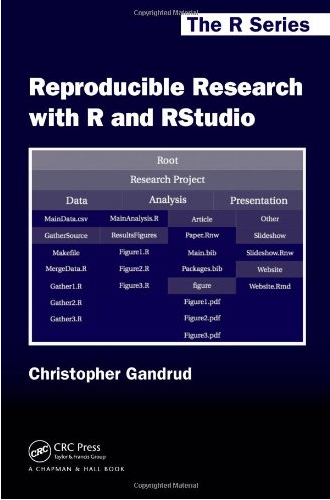
\includegraphics[width=0.6\columnwidth]{chris.png}
\end{figure}
\end{columns}

\end{frame}


\begin{frame}{Eat Your Own Dog Food}

\begin{itemize}
\item These slides are reproducible
\item Source code: \href{https://github.com/sahirbhatnagar/knitr-tutorial}{https://github.com/sahirbhatnagar/knitr-tutorial}
\end{itemize}

\end{frame}


\section{Reproducible Research}

\subsection{What?}

\begin{frame}

\frametitle{What is Science Anyway?}

\pause
\begin{block}{According to the American Physical Society:}
\emph{Science is the systematic enterprise of gathering knowledge about the universe and organizing and condensing that knowledge into \textbf{testable} laws and theories. The \textbf{success and credibility of science} are anchored in the \textbf{willingness} of scientists to \textbf{expose their ideas} and results to \textbf{independent testing} and \textbf{replication} by other scientists}
\end{block}

\end{frame}

%%%%%%%%%%%%%%%%%%%%%%%%%%%%%%%%%%%%%%%%%%%%%%%%%%%%%%%%%%%%%%%%%%%%%%%%%%%%%%%%%%%%%%%%%%%%%
\begin{frame}

\frametitle{RR: A Minimum Standard to Verify Scientific Findings}

\pause
\begin{block}{Reproducible Research (RR) in Computational Sciences}
\emph{The data and the code used to make a finding are available and they are sufficient for an independent researcher to recreate the finding}
\end{block}

\end{frame}

%%%%%%%%%%%%%%%%%%%%%%%%%%%%%%%%%%%%%%%%%%%%%%%%%%%%%%%%%%%%%%%%%%%%%%%%%%%%%%%%%%%%%%%%%%%%%
%%%%%%%%%%%%%%%%%%%%%%%%%%%%%%%%%%%%%%%%%%%%%%%%%%%%%%%%%%%%%%%%%%%%%%%%%%%%%%%%%%%%%%%%%%%%%

\subsection{Why?}

\begin{frame}
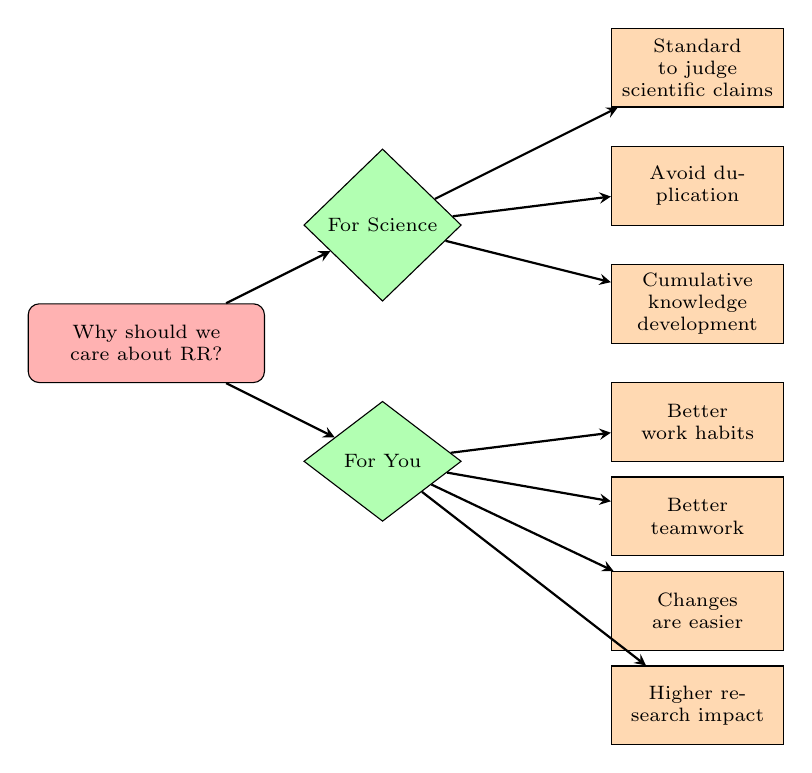
\begin{tikzpicture}
\scriptsize
\node (expr) [startstop] {Why should we care about RR?};
\node (science) [decision, right of=expr, xshift=2cm, yshift=1.5cm] {For Science};
\draw [arrow] (expr) -- (science);
\node (stan) [process, right of=science, xshift=3cm, yshift=2cm] {Standard to judge scientific claims};
\node (dupli) [process, right of=science, xshift=3cm, yshift=0.5cm] {Avoid duplication};
\node (know) [process, right of=science, xshift=3cm, yshift=-1cm] {Cumulative knowledge development};
\draw [arrow] (science) -- (stan);
\draw [arrow] (science) -- (dupli);
\draw [arrow] (science) -- (know);
\pause \node (you) [decision, right of=expr, xshift=2cm, yshift=-1.5cm] {For You};
\draw [arrow] (expr) -- (you);
\node (work) [process, right of=you, xshift=3cm, yshift=0.5cm] {Better work habits};
\node (team) [process, right of=you, xshift=3cm, yshift=-0.7cm] {Better teamwork};
\node (change) [process, right of=you, xshift=3cm, yshift=-1.9cm] {Changes are easier};
\node (soft) [process, right of=you, xshift=3cm, yshift=-3.1cm] {Higher research impact};
\draw [arrow] (you) -- (work);
\draw [arrow] (you) -- (team);
\draw [arrow] (you) -- (change);
\draw [arrow] (you) -- (soft);
\end{tikzpicture}
\end{frame}


\subsection{001-motivating-example}

\begin{frame}

\begin{table}
\begin{center}
\begin{scriptsize}
\begin{tabular}{l c c c }
\hline
                              & GLM & GLMM & GEE \\
\hline
Intercept                     & $\mathbf{2.64} \; [2.38;\ 2.90]^{*}$    & $\mathbf{2.20} \; [0.98;\ 3.41]^{*}$ & $\mathbf{3.55} \; [1.73;\ 5.36]^{*}$ \\
progabide                     & $-0.02 \; [-0.23;\ 0.19]$               & $-0.23 \; [-0.76;\ 0.30]$            & $-0.15 \; [-1.17;\ 0.88]$            \\
time                          & $-0.04 \; [-0.10;\ 0.01]$               & $-0.04 \; [-0.10;\ 0.01]$            & $-0.05 \; [-0.26;\ 0.16]$            \\
age                           & $\mathbf{-0.01} \; [-0.02;\ -0.01]^{*}$ & $-0.01 \; [-0.05;\ 0.03]$            & $-0.05 \; [-0.10;\ 0.01]$            \\
progabide:time                & $-0.03 \; [-0.11;\ 0.05]$               & $-0.03 \; [-0.11;\ 0.05]$            & $0.01 \; [-0.25;\ 0.26]$             \\
\hline
AIC                           & 3268.84                                 & 1403.91                              &                                      \\
BIC                           & 3286.16                                 & 1424.69                              &                                      \\
Log Likelihood                & -1629.42                                & -695.95                              &                                      \\
Deviance                      & 2492.94                                 &                                      &                                      \\
Num. obs.                     & 236                                     & 236                                  & 236                                  \\
Num. groups: subject          &                                         & 59                                   &                                      \\
Variance: subject.(Intercept) &                                         & 0.87                                 &                                      \\
Variance: Residual            &                                         & 1.00                                 &                                      \\
Num. clust.                   &                                         &                                      & 59                                   \\
\hline
\multicolumn{4}{l}{\tiny{$^*$ 0 outside the confidence interval}}
\end{tabular}
\end{scriptsize}
\caption{Comparing model estimates}
\label{table:coefficients}
\end{center}
\end{table}

\end{frame}


\section{002-tables}
\begin{frame}

% Table created by stargazer v.5.1 by Marek Hlavac, Harvard University. E-mail: hlavac at fas.harvard.edu
% Date and time: Mon, May 25, 2015 - 11:32:33 AM
\begin{table}[!htbp] \centering 
  \caption{} 
  \label{} 
\begin{tabular}{@{\extracolsep{5pt}}lc} 
\\[-1.8ex]\hline 
\hline \\[-1.8ex] 
 & \multicolumn{1}{c}{\textit{Dependent variable:}} \\ 
\cline{2-2} 
\\[-1.8ex] & mpg \\ 
\hline \\[-1.8ex] 
 wt & $-$5.30$^{***}$ \\ 
  & (0.56) \\ 
  & \\ 
 Constant & 37.00$^{***}$ \\ 
  & (1.90) \\ 
  & \\ 
\hline \\[-1.8ex] 
Observations & 32 \\ 
R$^{2}$ & 0.75 \\ 
Adjusted R$^{2}$ & 0.74 \\ 
Residual Std. Error & 3.00 (df = 30) \\ 
F Statistic & 91.00$^{***}$ (df = 1; 30) \\ 
\hline 
\hline \\[-1.8ex] 
\textit{Note:}  & \multicolumn{1}{r}{$^{*}$p$<$0.1; $^{**}$p$<$0.05; $^{***}$p$<$0.01} \\ 
\end{tabular} 
\end{table} 
numeric(0)

\end{frame}

\begin{frame}

\begin{table}
\begin{center}
\begin{scriptsize}
\begin{tabular}{l c c c }
\hline
                              & GLM & GLMM & GEE \\
\hline
Intercept                     & $\mathbf{2.64} \; [2.38;\ 2.90]^{*}$    & $\mathbf{2.20} \; [0.98;\ 3.41]^{*}$ & $\mathbf{3.55} \; [1.73;\ 5.36]^{*}$ \\
progabide                     & $-0.02 \; [-0.23;\ 0.19]$               & $-0.23 \; [-0.76;\ 0.30]$            & $-0.15 \; [-1.17;\ 0.88]$            \\
time                          & $-0.04 \; [-0.10;\ 0.01]$               & $-0.04 \; [-0.10;\ 0.01]$            & $-0.05 \; [-0.26;\ 0.16]$            \\
age                           & $\mathbf{-0.01} \; [-0.02;\ -0.01]^{*}$ & $-0.01 \; [-0.05;\ 0.03]$            & $-0.05 \; [-0.10;\ 0.01]$            \\
progabide:time                & $-0.03 \; [-0.11;\ 0.05]$               & $-0.03 \; [-0.11;\ 0.05]$            & $0.01 \; [-0.25;\ 0.26]$             \\
\hline
AIC                           & 3268.84                                 & 1403.91                              &                                      \\
BIC                           & 3286.16                                 & 1424.69                              &                                      \\
Log Likelihood                & -1629.42                                & -695.95                              &                                      \\
Deviance                      & 2492.94                                 &                                      &                                      \\
Num. obs.                     & 236                                     & 236                                  & 236                                  \\
Num. groups: subject          &                                         & 59                                   &                                      \\
Variance: subject.(Intercept) &                                         & 0.87                                 &                                      \\
Variance: Residual            &                                         & 1.00                                 &                                      \\
Num. clust.                   &                                         &                                      & 59                                   \\
\hline
\multicolumn{4}{l}{\tiny{$^*$ 0 outside the confidence interval}}
\end{tabular}
\end{scriptsize}
\caption{Comparing model estimates}
\label{table:coefficients}
\end{center}
\end{table}

\end{frame}



\end{document}
